The implementation of the project was done in python. In general classes containing logic for different objects were implemented, for instance classes for polynomials, factorials, powers and so on were implemented. All classes were implemented from scratch and we want to stress that this makes some of the code redundant -- surely it is implemented by others before -- and inefficient -- no highly efficient methods are used, but only the most simple versions. The reason the classes were implemented from scratch anyways was to more deeply understand the problems arising within computer algebra, and during the process it became clear that even methods that are very simple in theory can cause several hours of implementation and many lines of code.

The implementation of Wilf-Zeilberger's method can be divided into mainly three parts: parsing, testing and methods. Parsing is when we read a string and convert this into classes or logic that is used in the rest of the code. This is mainly to ease testing of the methods that are implemented but also for running the main program. Testing is when we test the methods and see that they behave as intended. Methods is the ''real'' code for the thesis, which is when we implement the logic that is described in chapter \ref{Ch: Theory}. In total the code produced in the thesis consists of about 2200 lines of code out of which about 50\% are the methods and classes used to implement the theory from chapter \ref{Ch: Theory}, 20\% is parsing and 30\% is testing. The testing is of course not necessary to keep for the sake of having functioning code, but is kept anyways in order to show that the code has been tested.

The code consists of eight files that do different parts of the method. These are:

\begin{center}
  \begin{tabular}{C{1mm}C{3cm}|C{8cm}}
    &\textbf{File name}   & \textbf{What does the file include?} \\ \hline
    &Polynomial  & A class for polynomials with all methods that are needed. \\ \hline
    &Factor      & Classes for factorials and powers (integer to the power of polynomials) \\ \hline
    &Expressions & Classes for storing expressions of factors, addends and fractional expressions \\ \hline
    &Main        & Main function that takes a parser and an input string as input and produces a \LaTeX-file with a part proof where the user only needs to do a few steps (which are indicated in the \LaTeX-file) \\ \hline
    &Gosper      & Functions for running all steps of Gosper's algorithm and returning the solution \\ \hline
    &Get f       & Function for solving step 2 of Gosper's algorithm \\ \hline
    &Gaussian elimination & Function for solving a system of linear equations by using Gaussian elimination, which is used by Get f \\ \hline
    &Parsers     & Parser from a \LaTeX equation to the format that is used in the rest of the program \\
  \end{tabular}
\end{center}

The dependencies of the files can be drawn as follows where an arrow from $A$ to $B$ means that $B$ depends on $A$:
\begin{figure}[H]
\centering
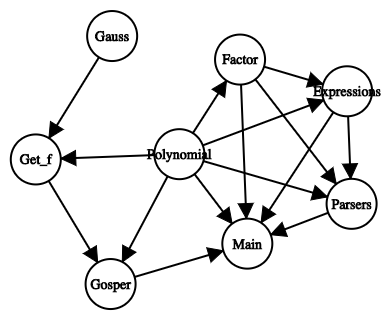
\includegraphics[width=0.6\textwidth]{images/dependency_graph.png}
\caption{Dependency graph of code}\label{Fig: DepGraph}
\end{figure}
Now that we have shown the general structure of the program, we will describe each of the important and interesting parts of the implementation. Firstly we will describe the structure used for parsing, thereafter we will discuss implementation of the methods needed for Wilf-Zeilberger's method. After that we will describe how a proof is written automatically and lastly we will describe how testing has been done.

\section{Parsing}
In the project several parsers are used. The parsers that have been implemented are shift-reduce parsers, which are a type of bottom-up parsers. In this type of parser a stack is used and a string is parsed character by character. When a character is read first the stack is reduced and then the character is pushed to the stack. That the stack is reduced means that if we read for instance a ''$+$'', then first all multiplications on the top of the stack are evaluated and after that we push the ''$+$''. For more details and further explanation of a shift-reduce parser, see \reference{parser}.

In the code there are four parsers, which all read a string of a specific format and return either an object that the string represents or a string on another format. We are now going to describe the parsers with what they have as input and output, but first we need to describe an internal format that is used in the program to represent binomial coefficients, factorials and powers of integers. This format will in the rest of the report be referred to as \textit{the internal format} These three will be represented as follows:
\begin{center}
  \begin{tabular}{C{1mm}C{3cm}|C{4cm}|C{4cm}}
    &\textbf{What?}   & \textbf{Represented as:} & \textbf{Example:} \\ \hline
    &Factorial & $F[x]$, where $x$ is a polynomial & $(m+n)!$ is written as $F[n+m]$ \\ \hline
    &Binomial coefficient & $B[n,k]$ where $n,k$ are polynomials & $\binom{n+1}{k-1}$ is written as $B[n+1,k-1]$ \\ \hline
    &Power of integer & $P[a,n]$ where $a$ is an integer and $n$ is a polynomial & $2^n$ is written as $P[2,n]$ \\
  \end{tabular}
\end{center}

The parsers are described by the following table:
\begin{center}
  \begin{tabular}{C{1mm}C{3cm}|C{4cm}|C{4cm}}
    &\textbf{Parser}   & \textbf{Input format} & \textbf{Output format} \\ \hline
    &Polynomial parser & String with a polynomial, for instance ''n\^{}2+3km'' & Polynomial that the input string represents \\ \hline
    &Expression parser & String with an expression on the internal format, for instance ''(n!+k*m)/(n\^{}2+B[n,k])'' & Expression that the input string represents \\ \hline
    &\LaTeX parser     & String in \LaTeX format of an identity, for instance ''\textbackslash sum\_\{k=0\}\^{}n \textbackslash binom\{n\}\{k\}=2\^{}n'' & $F, a_k$ and the numerator and denominator of $\frac{a_k}{a_{k-1}}$ as the first step in the method after which Gosper's algorithm can be run \\ \hline
    &Internal format to \LaTeX parser  & String on the internal format & String on \LaTeX format, which is used when generating the proof file \\
  \end{tabular}
\end{center}

\section{Gosper's algorithm}
Although the whole algorithm is described in section \ref{Sec: Gosper}, we will again go through the algorithm but from the perspective of implementation, and trying to point out difficulties along the way. There are some parts where the theory is straight forward, but the details in the implementation are quite difficult. In this section we try to describe the choices that were made during the work of the thesis, and also point out advantages and disadvantages with these choices.
\subsection{Finding p,q,r}
In section \ref{Sub: pqr} an algorithm is described for how to find polynomials $p,q,r$ such that
\begin{equation}\label{Eq: getpqr}
  \frac{a_k}{a_{k-1}} = \frac{p_k}{p_{k-1}}\frac{q_k}{r_k},
\end{equation}
such that $gcd(q_k,r_{k+j})=1 \forall j\geq 0$. The algorithm can be described as follows:
\begin{algorithm}[H]
  \caption{Get $p,q,r$}
  \inp{Rational polynomial $b=\frac{b_n}{b_d}=\frac{a_k}{a_{k-1}}$}
  \outp{Polynomials $p,q,r$ such that \ref{Eq: getpqr} holds and $gcd(q_k,r_{k+j})=1\forall j\geq 0$}
  \begin{algorithmic}[1]
    \Procedure{getpqr}{$b_n,b_d$}
      \State $r_k\gets b_d$
      \State $q_k\gets b_n$
      \State $p_k\gets 1$
      \While{$\exists j\geq 0: gcd(q_k,r_{k+j})\neq 1$}
        \State $j\gets j \text{ such that } gcd(q_k,r_{k+j})\neq 1$
        \State $g_k\gets gcd(q_k,r_{k+j})$
        \State $q_k\gets \frac{q_k}{g_k}$
        \State $r_k\gets \frac{r_k}{g_{k-j}}$
        \State $p_k\gets p_kg_kg_{k-1}\ldots g_{k-j+1}$
      \EndWhile
      \State \Return $p_k,q_k,r_k$
    \EndProcedure
  \end{algorithmic}
\end{algorithm}
This algorithm is in theory fairly simple -- find a common factor and get rid of it -- but finding $gcd(q_k,r_{k+j})$ for all $j$ and see if this can be a common factor is tricky implementationwise. In the thesis this is implemented in the following fashion:
\begin{algorithm}[H]
  \caption{Find $GCD(q_k,r_{k+j})\forall j\geq 0$}
  \inp{Polynomials $q_k,r_k$}
  \outp{Polynomial $g_k=gcd(q_k,r_{k+j})$ for some $j\geq 0$}
  \begin{algorithmic}[1]
    \Procedure{GCDWithShift}{$q_k,r_k$}
      \State $g_{j,0}\gets r_k \text{ evaluated at } k=k+j$
      \State $g_{j,1}\gets \Call{GCD}{q_k,g_{j,0}}$
      \State $i\gets 1$
      \While{$g_{j,i}\neq 1$}
        \If{$\exists j^\prime\geq 0: g_{j,i}(j^\prime)=0$}\label{Alg: GCDWithShift,if}
          \State \Return $j^\prime$
        \EndIf
        \State $i\gets i+1$
        \State $g_{j,i}\gets \Call{GCD}{g_{j,i-2},g_{j,i-1}}$
      \EndWhile
      \State \Return $None$
    \EndProcedure
  \end{algorithmic}
\end{algorithm}
Here we perform the check in the if-statement on line \ref{Alg: GCDWithShift,if} by calling procedure \ref{Alg: Roots} and then checking if there is any root that is positive. Since this is the crucial step of this algorithm both the advantages and disadvantages come from the Roots-algorithm. In the implementation of Roots, only up to second degree polynomials are solved completely and after that values in the interval $(-100,100)$ are tested. This means that we cannot be sure that we find the roots. In general when we can use Wilf-Zeilberger's method, however, all roots are fairly small -- almost always less than 100. Therefore even though the implementation in theory is limiting it is very likely not to cause any problems in practice.
\subsection{Finding f}
The implementation in order to find the polynomial $f$ in Gosper's algorithm is performed just as described in section \ref{Sub: getf}. The goal of that is to find $f$ such that
\begin{equation}\label{Eq: getf}
  p_k=q_{k+1}f_k-r_kf_{k-1}.
\end{equation}
First the matrix $M$ and the vector $P$ are constructed. $M$ comes from the right hand side of \ref{Eq: getf} after assigning $f$ as stated in equation \ref{Eq: Theory,general polynomial}. $P$ is the vector that represent the coefficients on the left hand side. After the construction, Gaussian elimination is performed and then hopefully an answer will be given.

In case no answer has been found one can try to increase the maximal degree of $f$. It is not certain however that a solution can be given by this method since possibly the degree of the smallest degree solution for $f$ can be arbitrarily large with respect to the variables that are not $k$. If a solution is given, however, then we have performed the whole Gosper's algorithm.

\section{Proof generation}
The proof generation is a method which needs an input string and a parser. Then the method produces a proof, written in \LaTeX code, for that the input string in fact is true. Right now the parser that has been developed in the thesis can only handle a few different types of operators in the input string -- binomial coefficients, factorials, integer powers and polynomials can be handled, but no other operators. The reason for this is that the parser mostly is an example of how Wilf-Zeilberger's method can be used, and is not meant to be a full solution. Instead users can write their own parsers and input strings which convert the string into four things: $F,a_k$ and the numerator and denominator of the fraction $\frac{a_k}{a_{k-1}}$. When the user has provided this parser and input string, then the main-function does the rest of the job in producing the proof in \LaTeX format, which proves the identity.

The reasons for this design choice (to only provide a simple parser as an example) are a few: firstly this gives a flexibility for a user and works well in an open source setting, secondly it would be at least as time demanding as writing the rest of the method to write a more general parser for more kinds of identity parsing -- and still some applications would probably be left out anyways.

The general methodology used in the proof generation is the following:
\begin{enumerate}[i)]
  \item Get a parser and an input string as inputs.
  \item Parse the string, which gives us $F,a_k$ and the polynomials that are the numerator and denominator of $\frac{a_k}{a_{k-1}}$.
  \item Call Gosper's algorithm which gives a $G(n,k)$ such that $G(n,k+1)-G(n,k)=a_k=F(n+1,k)-F(n,k)$. This step is the main contribution from the program, and is usually the by far hardest part of the proof.
  \item Write the proof in \LaTeX format.
  \item Highlight parts of the proof that need to be verified or partly proved by the user. This includes proving that $\lim_{k\to\pm\infty}G(n,k)=0\forall n$ and may include verifying that $G(n,k+1)-G(n,k)=F(n+1,k)-F(n,k)$. This should be guaranteed by the solver, but might be worth verifying.
\end{enumerate}
\section{Testing}
In general the testing has tried to test each method individually and then first after each methods works on its own it has been tested all together. The testing on each individual method has been performed in different ways for different methods, but the common thing for all of the methods is that the testing included many edge cases as well as other cases. Edge cases are usually when some parameters (for instance the degree of a polynomial or the number of variables in the polynomial) is very small or large.

The tests that were performed on methods all together are usually from one of the test examples provided in chapter \ref{Ch: Results}. Then the implementation and testing was iterated until all identities worked. This testing was also performed in steps, for instance in order to test the methods in Gosper's algorithm, some initial steps were done by hand and then the relevant part was tested. Then, when all individual methods and groups of methods worked as expected, everything was put together and the final result was given.
